\chapter{Procedure}

\section{Analytical Calculations in Phasor Domain}

\subsection{Determine the Capacitor Value}

\begin{figure}[h]
    \centering
    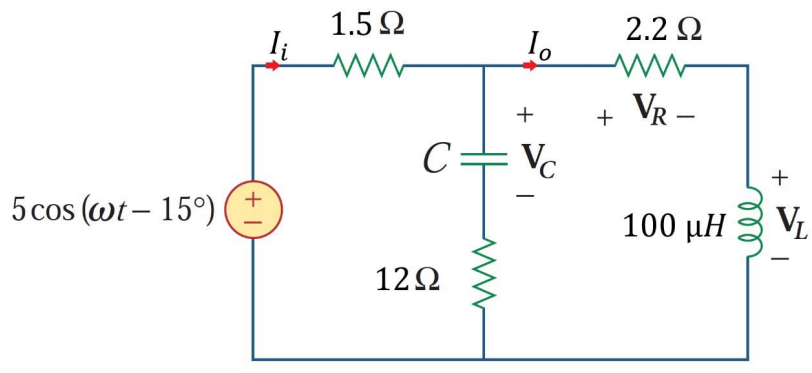
\includegraphics[width=0.5\textwidth]{assets/circuit.png}
    \caption{RLC Circuit}
    \label{fig:rlc-circuit}
\end{figure}

Transforming this circuit into the phasor domain, we have the following circuit:

\begin{figure}[h]
    \centering
    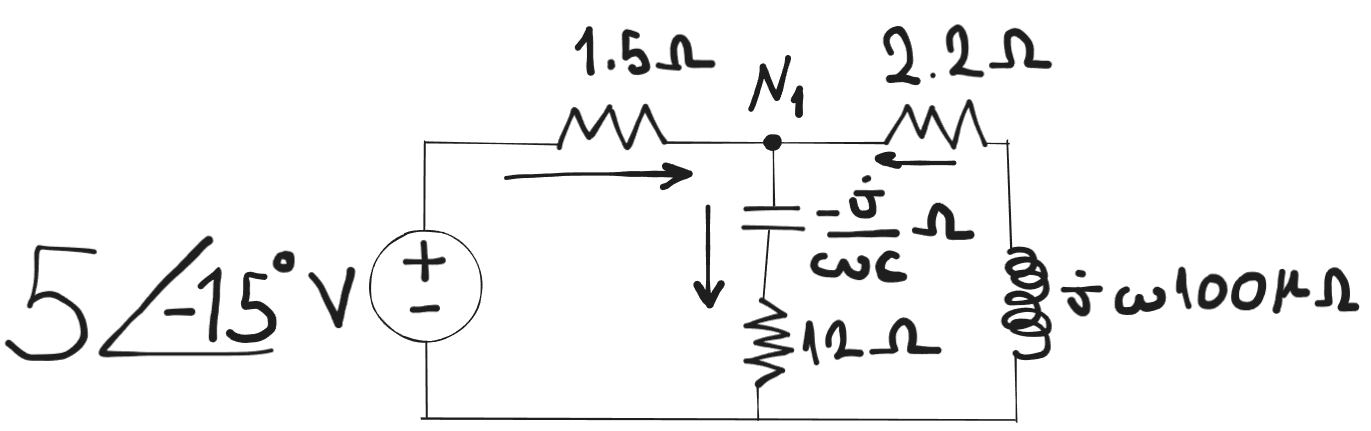
\includegraphics[width=0.7\textwidth]{assets/circuit-phasor.png}
    \caption{RLC Circuit Phasor Domain}
    \label{fig:rlc-circuit-phasor}
\end{figure}

Applying nodal analysis at node $N_{1}$:

\begin{equation}
    \frac{V_S - N_1}{1.5} + \frac{N_1}{2.2 + j 2\pi \times 10^{-1}} - \frac{N_1}{12 + \frac{-j}{2000\pi C}} = 0
\end{equation}

$V_S$ and $N_1$ are given as $V_S = 5 \angle{-15^{\circ}}$ and $N_1 = 2 \angle{-7.5^{\circ}}$.

\newpage
\thispagestyle{plain}

Solving for $C$:

\begin{equation}
    \frac{5 \angle{-15^{\circ}} - 2 \angle{-7.5^{\circ}}}{1.5} + \frac{2 \angle{-7.5^{\circ}}}{2.2 + j 2\pi \times 10^{-1}} - \frac{2 \angle{-7.5^{\circ}}}{12 + \frac{-j}{2000\pi C}} = 0
\end{equation}

\begin{equation}
    \frac{5 \angle{-15^{\circ}} - 2 \angle{-7.5^{\circ}}}{1.5} + \frac{2 \angle{-7.5^{\circ}}}{2.2 + j 2\pi \times 10^{-1}} = \frac{2 \angle{-7.5^{\circ}}}{12 + \frac{-j}{2000\pi C}}
\end{equation}

\begin{equation}
    2.0189 \angle{-19.9451^{\circ}} + 0.8741 \angle{-23.4393^{\circ}} = \frac{2 \angle{-7.5^{\circ}}}{12 + \frac{-j}{2000\pi C}}
\end{equation}

\begin{equation}
    2.8919 \angle{-21.0007^{\circ}} = \frac{2 \angle{-7.5^{\circ}}}{12 + \frac{-j}{2000\pi C}}
\end{equation}

\begin{equation}
    \frac{-j}{2000\pi C} = \frac{2 \angle{-7.5^{\circ}}}{2.8919 \angle{-21.0007^{\circ}}} - 12 = 11.3287 \angle{179.1834^{\circ}}
\end{equation}

\begin{equation}\label{eq:capacitor-value}
    C = \frac{-j}{2000\pi \times 11.3287 \angle{179.1834^{\circ}}} = 1.4049 \angle{90.8166^{\circ}} = -200.2236 \times 10^{-9} + j14.0474 \times 10^{-6}
\end{equation}

From equation \ref{eq:capacitor-value}, we have $C = -200.2236 \times 10^{-9} + j14.0474 \times 10^{-6}$, which means there should be a capacitor with a real value which is impossible. Therefore, we can add a $200.2236 \times 10^-9 \Omega$ resistor in series to the capacitor to make it only capacitive. After that, the capacitor value is $j14.0474 \mu \Omega$.

\subsection{Calculating Voltage and Current Values}

After finding the capacitor value, we know everything about the circuit. We can calculate the Voltage and current values as follows:

\begin{equation}\label{eq:current-out}
    I_O = \frac{2\angle{-7.5^{\circ}}}{2.2 + j 2\pi \times 10^{-1}} = 0.802 \angle{-3.4771^{\circ}} A
\end{equation}

\begin{equation}\label{eq:current-in}
    I_i = \frac{5\angle{-15^{\circ}} - 2\angle{-7.5^{\circ}}}{1.5} = 2.0189 \angle{-19.9451^{\circ}} A
\end{equation}

\begin{equation}\label{eq:current-capacitor}
    I_C = I_i - I_O = 1.2703\angle{-30.255^{\circ}} A
\end{equation}

And from the current values, we can calculate the voltage values:

\begin{equation}\label{eq:voltage-resistor}
    V_R = I_O \times 2.2 = 1.7644 \angle{-3.4771^{\circ}} V
\end{equation}

\begin{equation}\label{eq:voltage-inductor}
    V_L = I_O \times j 2\pi \times 10^{-1} = 0.50391 \angle{86.5229^{\circ}} V
\end{equation}

\begin{equation}\label{eq:voltage-capacitor}
    V_C = I_C \times j14.0474\mu = 1.7844\angle{59.745^{\circ}}V
\end{equation}

\newpage
\thispagestyle{plain}

Converting the phasor voltages and currents to time domain:

\begin{equation}\label{eq:voltage-resistor-time}
    v_R(t) = 1.7644 \cos(2000\pi t - 3.4771^{\circ}) V
\end{equation}

\begin{equation}\label{eq:voltage-inductor-time}
    v_L(t) = 0.50391 \cos(2000\pi t + 86.5229^{\circ}) V
\end{equation}

\begin{equation}\label{eq:voltage-capacitor-time}
    v_C(t) = 1.7844 \cos(2000\pi t + 59.745^{\circ}) V
\end{equation}

\begin{equation}\label{eq:current-out-time}
    i_O(t) = 0.802 \cos(2000\pi t - 3.4771^{\circ}) A
\end{equation}

\begin{equation}\label{eq:current-in-time}
    i_i(t) = 2.0189 \cos(2000\pi t - 19.9451^{\circ}) A
\end{equation}

\begin{equation}\label{eq:current-capacitor-time}
    i_C(t) = 1.2703 \cos(2000\pi t - 30.255^{\circ}) A
\end{equation}

\newpage
\thispagestyle{plain}

\section{SPICE Simulation}

\begin{figure}[h]
    \centering
    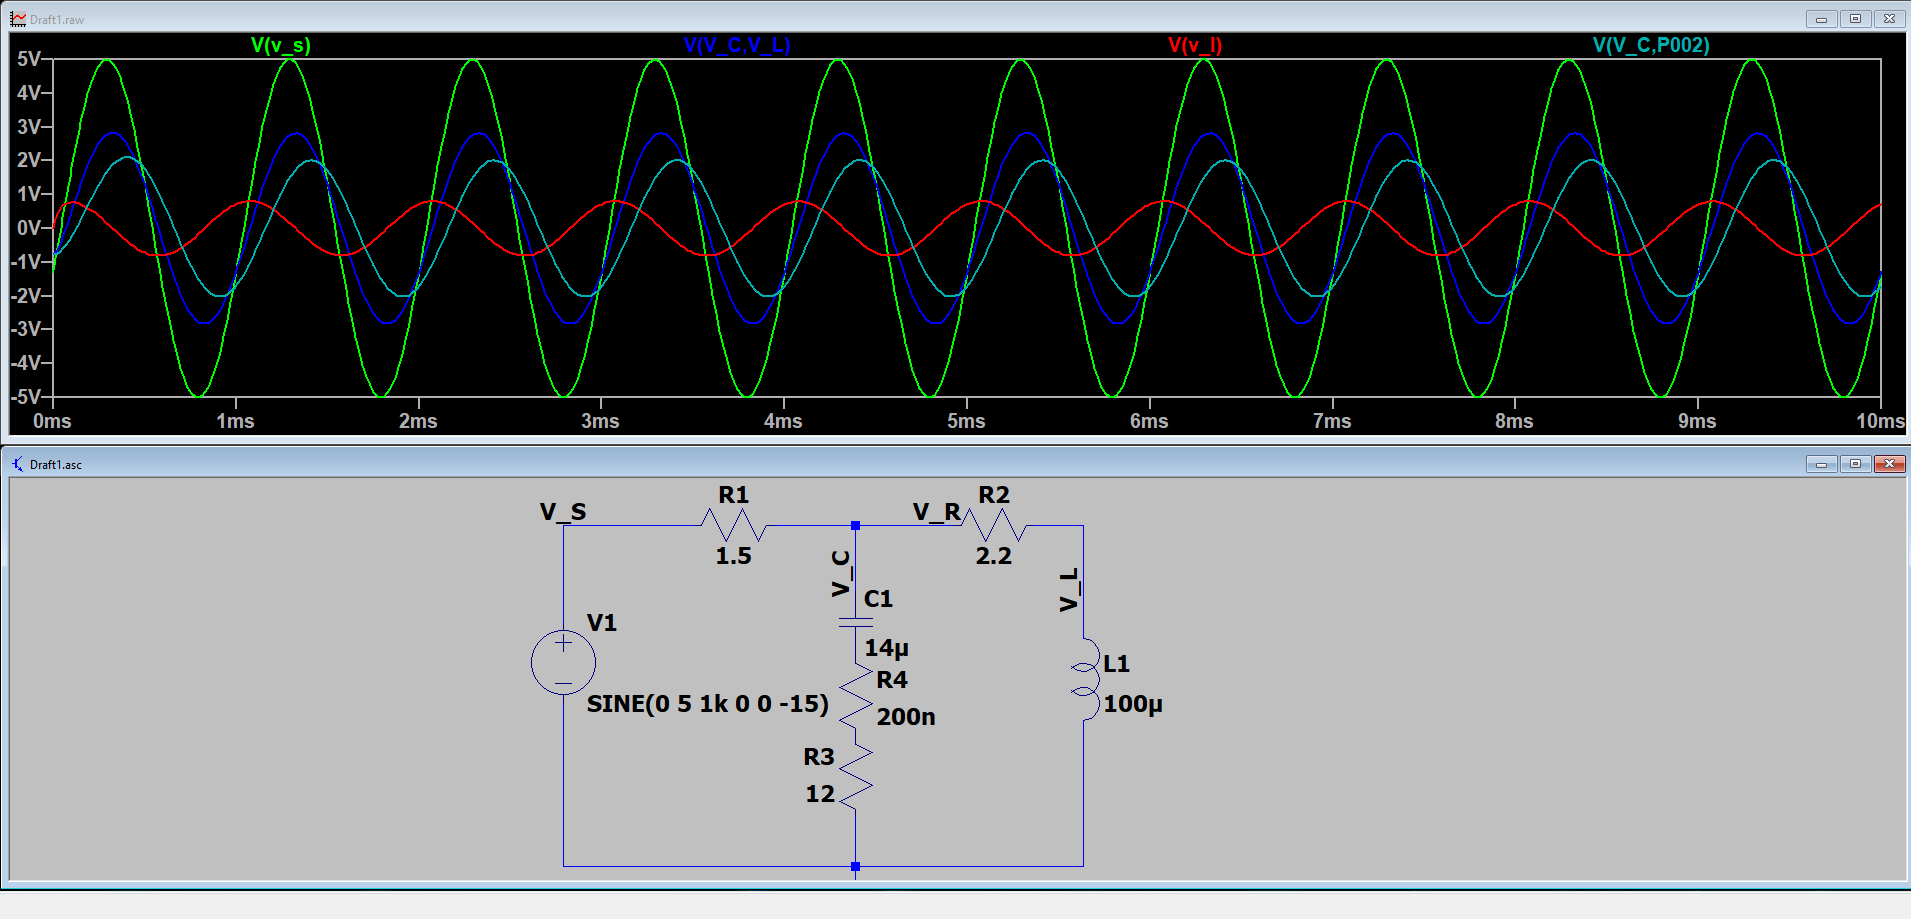
\includegraphics[width=1\textwidth]{assets/sim-voltage.png}
    \caption{SPICE Voltage Simulation}
    \label{fig:spice-circuit}
\end{figure}

\begin{figure}[h]
    \centering
    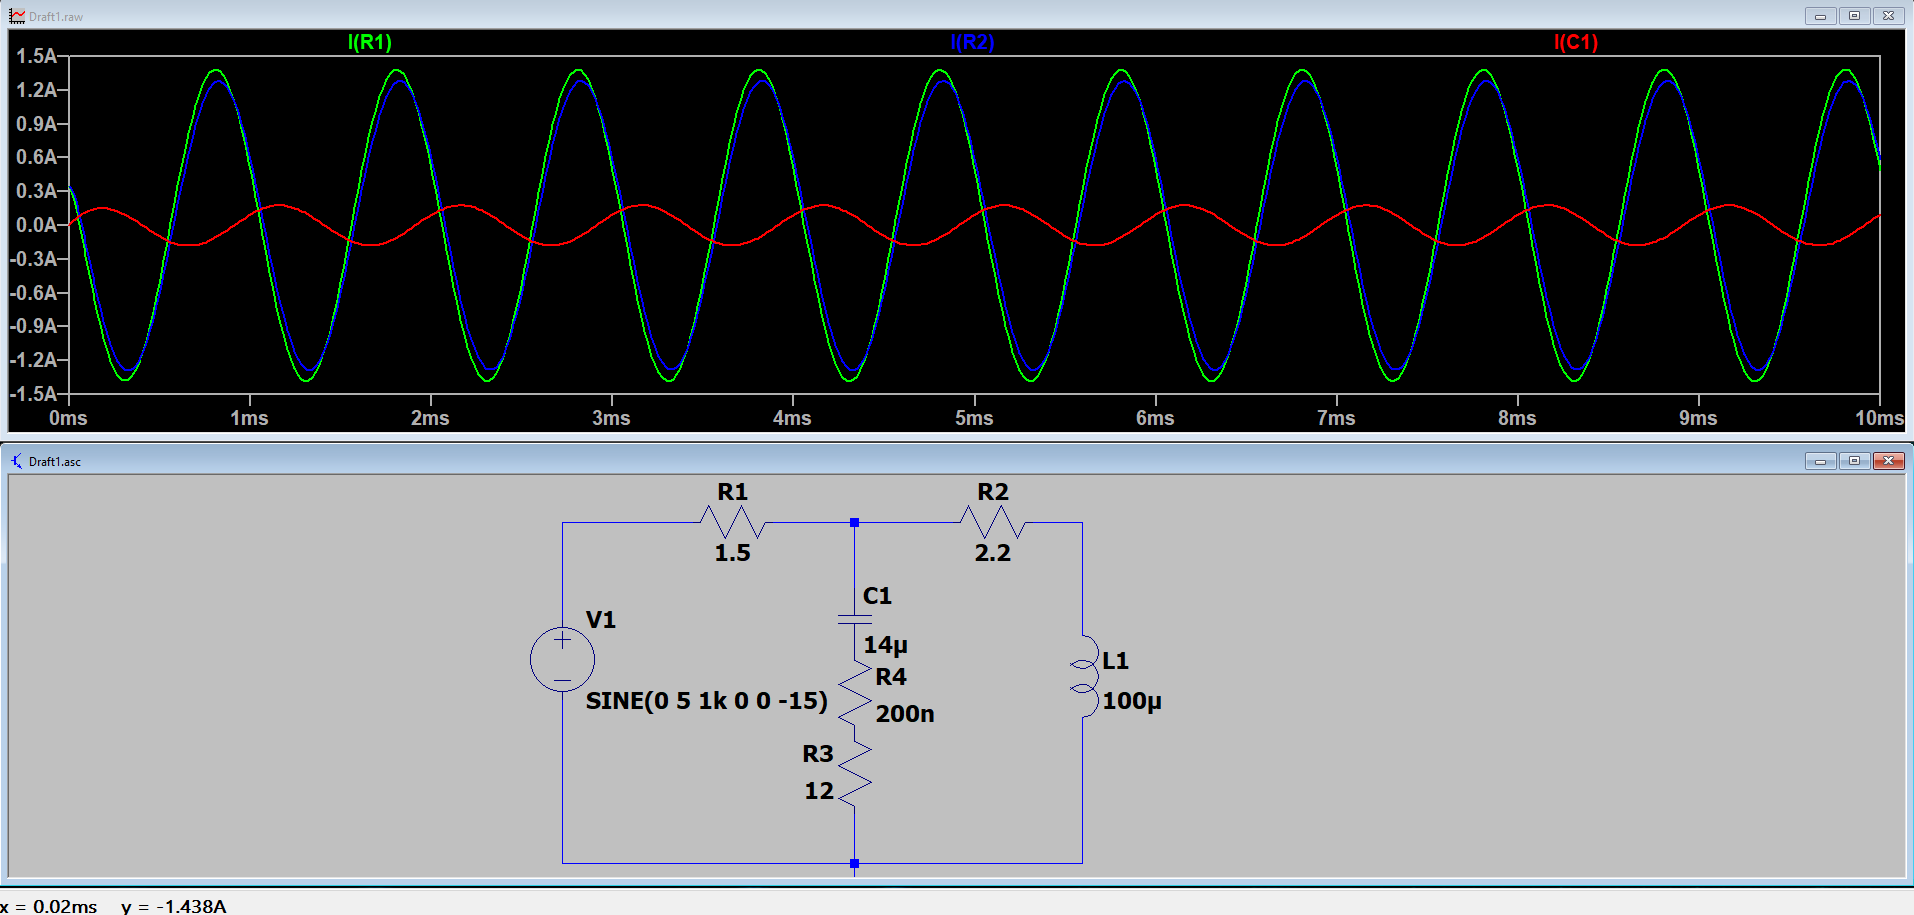
\includegraphics[width=1\textwidth]{assets/sim-current.png}
    \caption{SPICE Current Simulation}
    \label{fig:spice-circuit}
\end{figure}

Comparing the SPICE simulation results with the analytical calculations, everything seems to be correct.

